\section{Bibliotheken}
\subsection{NumPy}
NumPy ist eine Bibliothek für Python, die diverse Features unterstützt, die wissenschaftliches Arbeiten deutlich erleichtern.
Einige davon sind
\begin{itemize}
  \item ein $n$-dimensionales Array-Objekt
  \item ausgeklügelte, durchdachte Funktionen für Optimierung, Integration und Interpolation
  \item die Möglichkeit C/C++- und Fortran-Code zu integrieren
  \item Tools für Lineare Algebra, Fouriertransformation, Statistik
  \item beliebige eigene Datentypen können definiert werden
\end{itemize}

\subsection{SciPy}
SciPy ist, ähnlich wie NumPy, eine Bibliothek, die wissenschaftliches Arbeiten erleichtert.
Insbesondere sind in dem Paket verschiedene Konstanten gespeichert, die im Praktikum oft gebraucht werden.
SciPy ist eine Erweiterung von NumPy, die vor allem vom NumPy-Array profitiert.
Es besitzt ebenfalls viele benutzerfreundliche und effiziente numerische Algorithmen für Integration und Optimierung.

\subsection{matplotlib}
Bei matplotlib handelt es ich um eine Bibliothek für Plots.
\begin{quote}
  \textit{matplotlib tries to make easy things easy and hard things possible.}
\end{quote}
Es dient dazu Plots, auch polare, sowie Fehlerbalken und noch vieles mehr zu Plotten.
Es bietet sehr viele Einstellungsmöglichkeiten mit denen man den Plot anpassen kann.
matplotlib bietet eine objektorientierte API, die erlaubt die Plots in Anwendungen einzubetten die generische GUI-Toolkits wie Qt oder GTK benutzen.
Es gibt ebenfalls PyLab, das die verwendung in IPython erleichtert.

\subsubsection{Objektorientiertes Interface}
\begin{figure}[H]
  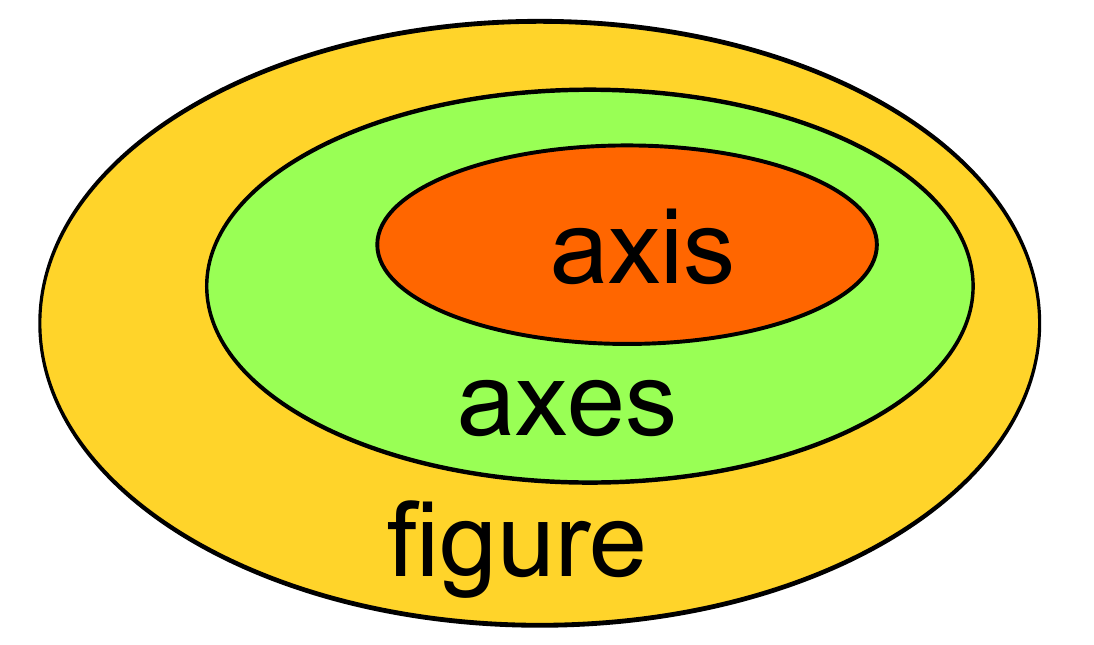
\includegraphics[width=150px]{img/matplotlib_v.png}
\end{figure}
\begin{itemize}
  \item figure: Leinwand, auf die Plots projiziert werden
  \item axes: enthält Plot, der beliebig in der figure plaziert werden kann
  \item axis: Koordinatenachsen 
\end{itemize}

\subsubsection{Linienstyles und Farben}
Die Übersichten in \autoref{tab:plt_lines} und \autoref{tab:plt_colors} stammen von \url{http://www.thetechrepo.com/main-articles/469-how-to-change-line-properties-in-matplotlib-python}.

\begin{table}[H]
  \centering{}
  \caption{Linienstile}
  \label{tab:plt_lines}
  \begin{tabular}{c l}
    \toprule
      Buchstabe & Stil \\
    \midrule
      \texttt{-} & solid line style \\
      \texttt{--} & dashed line style \\
      \texttt{-}. &  dash-dot line style \\
      \texttt{:} & dotted line style \\
      \texttt{.} & point marker \\
      \texttt{,} & pixel marker \\
      \texttt{o} & circle marker \\
      \texttt{v} & triangle\_down marker \\
      \texttt{\^{}} & triangle\_up marker \\
      \texttt{<} & triangle\_left marker \\
      \texttt{>} & triangle\_right marker \\
      \texttt{1} & tri\_down marker \\
      \texttt{2} & tri\_up marker \\
      \texttt{3} & tri\_left marker \\
      \texttt{4} & tri\_right marker \\
      \texttt{s} & square marker \\
      \texttt{p} & pentagon marker \\
      \texttt{*} & star marker \\
      \texttt{h} & hexagon1 marker \\
      \texttt{H} & hexagon2 marker \\
      \texttt{+} & plus marker \\
      \texttt{x} & x marker \\
      \texttt{D} & diamond marker \\
      \texttt{d} & thin\_diamond marker \\
      \texttt{|} & vline marker \\
      \texttt{\_} & hline marker \\
    \bottomrule
  \end{tabular}
\end{table}

\begin{table}[H]
  \centering{}
  \caption{Farben}
  \label{tab:plt_colors}
  \begin{tabular}{c l}
    \toprule
      Buchstabe & Farbe \\
    \midrule
      \texttt{k} & schwarz \\
      \texttt{w} & weiß \\
      \texttt{r} & rot \\
      \texttt{g} & grün \\
      \texttt{b} & blau \\
      \texttt{c} & cyan \\
      \texttt{y} & gelb \\
      \texttt{m} & magenta \\
    \bottomrule
  \end{tabular}
\end{table}

